This chapter presents a conceptual overview of SDR systems. \autoref{fig:sdr_block_diagram} shows a block diagram of a typical SDR system both from transmitter and receiver sides.
\begin{figure}[ht]
  \centering
  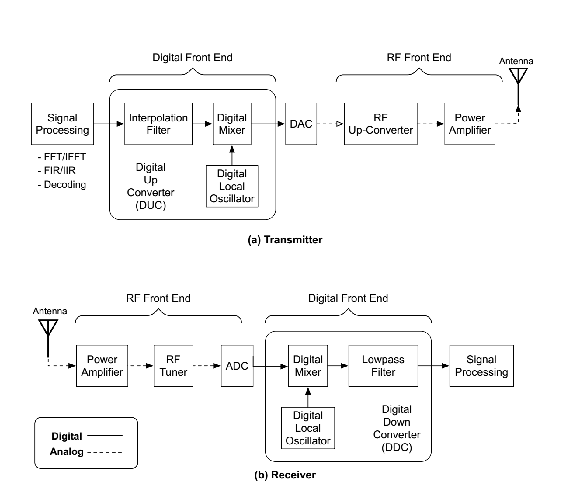
\includegraphics[width=0.75\textwidth]{sdr_block_diagram}
  \caption{Generic SDR architecture [\citeauthor{DBLP:journals/corr/abs-1804-06564}]}
  \label{fig:sdr_block_diagram}
\end{figure}

As shown, at a high level, an SDR transceiver typically consists of the following components: signal processing, digital front end, analogue RF front end, and an antenna.
\begin{enumerate}
  \item Antenna: Given one of the main requirements for SDR platforms is protocol flexibility, they usually employ several antennas to cover a wide range of frequency bands \cite{communications_receivers}. Other technologies that can be very useful in SDR systems are the so called `intelligent' or `smart' antennas due to their ability to select multiple frequency bands and adapt, using mobile tracking (i.e beam-forming capability), and/or interference cancellation (sometimes known as self-healing) \cite{rf_dig_sig_processing} \cite{review_tech_sdr}.

  \item RF front end: This is the RF circuitry responsible for transmitting and receiving the signal at various carrier frequencies. Its operation can briefly be summarized as follows:
  \begin{enumerate}
    \item In the transmission path, digital samples are converted into an analogue signal by the digital-to-analogue converter (DAC), which in turn feeds the RF front end. This analogue signal is mixed with a local oscillator (LO) signal to produce the RF signal at the preset frequency. It is then amplified using a power amplifier (PA) and transmitted. Advanced techniques such as digital pre-distortion (DPD) or envelope tracking, can be used to maximize output power while maintaining linearity in the PA. Other components that are typically part of this section are impedance matching networks, diplexers and RF filters such as surface acoustic wave (SAW) filters to reduce interference and comply with regulations like, for example, transmission masks.
    \item After being captured by the antenna, the signal is connected to the RF front end using a matching circuitry to guarantee an optimum signal power transfer. It then passes through a low noise amplifier (LNA), which resides in a close proximity to the antenna, to amplify weak signals and minimize the noise level. This amplified signal is mixed with the LO signal to produce a down-converted IF signal \cite{tech_radio_handbook}. Other components that can also exist are power detectors for gain control, and RF filters to suppress interference in the form of image frequencies.
  \end{enumerate}

  \item Analogue-to-digital (ADC) and digital-to-analogue (DAC) conversion: The DAC, as already mentioned, is responsible for producing the analogue signal to be transmitted, from the digital samples. On the receiver side, the ADC performs the inverse operation by converting the continuous-time signal to a discrete-time, binary-coded signals. ADC performance can be described by various parameters \cite{adc_survey} \cite{digital_frontend_sdr} including: signal-to-noise-and-distortion ratio (SINAD), effective number of bits resolution (ENOB), spurious-free dynamic range (SFDR), among others. These parameters are discussed in more detail, in \autoref{sect:radio_performance_and_impairment}.

  \item Digital front end: The digital front end has two main functions \cite{digital_frontend_sdr}:
  \begin{enumerate}
    \item  Sample rate conversion. Frequently, baseband blocks operate at a much lower frequency than the ADC/DAC devices. This requires an upsampling and interpolation operation (increasing the sample rate), or a decimation and downsampling operation (reducing the sample rate). The decimation filter in the receiver is typically matched to the transmitter's interpolation filter, in order to reduce additive noise. This is known as \emph{matched filtering} and is a common technique to design optimum receiving filters \cite{communication_systems_carlson}.
    \item Channelization. This includes up/down conversion in the transmitter and receiver side. In the transmitting side the digital up converter (DUC) translates the baseband signal to IF, using digital mixer and a numerically-controlled oscillator (NCO). The DAC that is connected to the DUC then converts the digital IF samples into an analogue IF signal. In the receiving side the ADC converts the IF signal into digital samples. These samples are subsequently fed into the next block, which is the digital down converter (DDC). The DDC includes a digital mixer and a NCO to obtain baseband digital signal from the IF signal, which is then forwarded to a high-speed digital signal processing block.
  \end{enumerate}

  \item Signal processing: Signal processing operations, such as encoding/decoding, interleaving/deinterleaving, modulation/demodulation, and scrambling/descrambling, are performed in this block. Encoding for the channel serves as an error correcting code. Specifically, the encoded signal includes redundancy that is used by the receiver's decoder to reconstruct the original signal from the corrupted received signal. Examples of error correcting codes include convolutional codes, turbo codes, and low density parity check (LDPC) \cite{crc_for_short_control_frames}. The decoder constitutes the most computationally intensive part of the signal processing block, due to data transfer and memory schemes \cite{channel_decoder_architecture}. The second part that is regarded as highly complex and expensive (in terms of area and power) is the fast Fourier transform (FFT) and inverse FFT (IFFT), which can be used in modulation (for example in orthogonal frequency-division multiplexing (OFDM) systems \cite{ofdm_baseband_receiver}) and other algorithms that operate in the frequency domain. The signal processing block is commonly referred to as the \emph{baseband processing block}. When discussing SDRs, the baseband block is at the heart of the discussion, as it makes up the bulk of the digital domain of the implementation. This implementation runs on top of a hardware circuitry that is capable of processing signals efficiently. Examples of these hardware platforms include general purpose processors (GPPs), graphics processing units (GPUs), digital signal processors (DSPs), field programmable gate arrays (FPGAs) and application-specific integrated circuits (ASICs). The second part of the implementation is the software, which provides the functionality and high-level abstractions to execute signal processing operations. In \autoref{sect:dsp_realizations} a more detailed discussion is presented on the aforementioned hardware platforms and the various design approaches.
\end{enumerate}

The next sections will be dedicated to describing each of the aforementioned SDR sections in more detail (with the exception of the antenna). Prior to that, in \autoref{sect:radio_performance_and_impairment}, a description is made of some general concepts related to radio performance and impairments, which are important to understand both the characteristics of each SDR architecture, and the results from the applications developed in \autoref{chap:demo_apps}. This section also discusses important parameters related to the ADC/DAC devices. \autoref{sect:sdr_system_architecture} then describes some of the possibilities for SDR topologies in terms of the RF front end and digital front end sections, listing their advantages and disadvantages. These topologies are broadly grouped into three groups:
\begin{enumerate}
  \item RF sampling: architectures which sample the RF signal directly, without first converting to an intermediate frequency or to baseband.
  \item IF sampling: architectures which first convert the signal to an intermediate frequency (usually in the tens of megahertz) and then perform sampling.
  \item Baseband sampling: Architectures which convert the signal to baseband (also known as 0 Hz or DC), and then perform sampling.
\end{enumerate}


Finally, \autoref{sect:dsp_realizations} discusses some of the most common options employed for realization of the signal processing stage (the core of the SDR), describing the advantages and disadvantages of each one.

%%%%%%%%%%%%%%%%%%%%%%%%%%%%%%%%%%%%%%%%%%%%%%%%%%%%%%%%%%%%%%%%%%%%%%%%%%%%%%%
\section{Radio Performance and Impairments}
\label{sect:radio_performance_and_impairment}

This sections describes some RF performance concepts and parameters, which are important when understanding the different SDR architectures, and when evaluating the performance of the developed algorithms and applications.

One of the most important parameters is the \emph{signal-to-noise ratio} (SNR) which defined as the ratio of the total signal power to the total noise power:
\begin{align}
  \text{SNR} = \frac{S}{N} = \left(\frac{S_{rms}}{N_{rms}}\right)^2
\end{align}
where
\begin{itemize}
  \item $S$ = Input signal power, in Watt
  \item $N$ = Noise power, in Watt
  \item $S_{rms}$ = Root-mean-square (RMS) amplitude of input signal
  \item $N_{rms}$ = RMS amplitude of noise
\end{itemize}

\noindent Power, noise and SNR are often expressed in logarithmic units, rather than linear units:
\begin{align}
  \text{SNR(dB)} = 10\log(SNR) =  10\log(S) - 10\log(N) = S\text{(dBm)} - N\text{(dBm)}
\end{align}

When analysing SDR systems, two of the most important components are ADC and the DAC. To analyse these, a common set of parameters is typically employed by manufacturers, which facilitates comparison between devices (although sometimes insufficient testing conditions information, such as signal frequency range, bandwidth and repetition, makes it difficult to obtain a trustworthy comparison). One of these parameters is the \emph{total harmonic distortion} (THD), which is defined as the ratio of the RMS value of the fundamental signal to the equivalent RMS of its harmonics (generally, only the first 5 harmonics are significant). THD of an ADC is usually measured in dBc and generally specified with the input signal close to full-scale, although it can be specified at any level.
\begin{align}
  \text{THD} = \frac{S_{rms}}{D_{rms}} = \frac{S_{rms}}{\sqrt{H_{1_{rms}}^2+H_{2_{rms}}^2+H_{3_{rms}}^2+H_{4_{rms}}^2+H_{5_{rms}}^2}}
\end{align}
where $D_{rms}$ represents distortion introduced by the harmonics.

\emph{Spurious free dynamic range} (SFDR) is another parameter, defined as the ratio of the RMS value of the input signal to the RMS value of the worst spurious signal regardless of where it falls in the frequency spectrum. The worst spur may or may not be a harmonic of the original signal. SFDR is an important specification in communications systems because it represents the smallest value of signal that can be distinguished from a large interferer. SFDR can be specified with respect to full-scale (dBFS) or with respect to the actual signal amplitude (dBc). \autoref{fig:sfdr_plot} illustrates how SFDR can be measured.

\begin{figure}[ht]
  \centering
  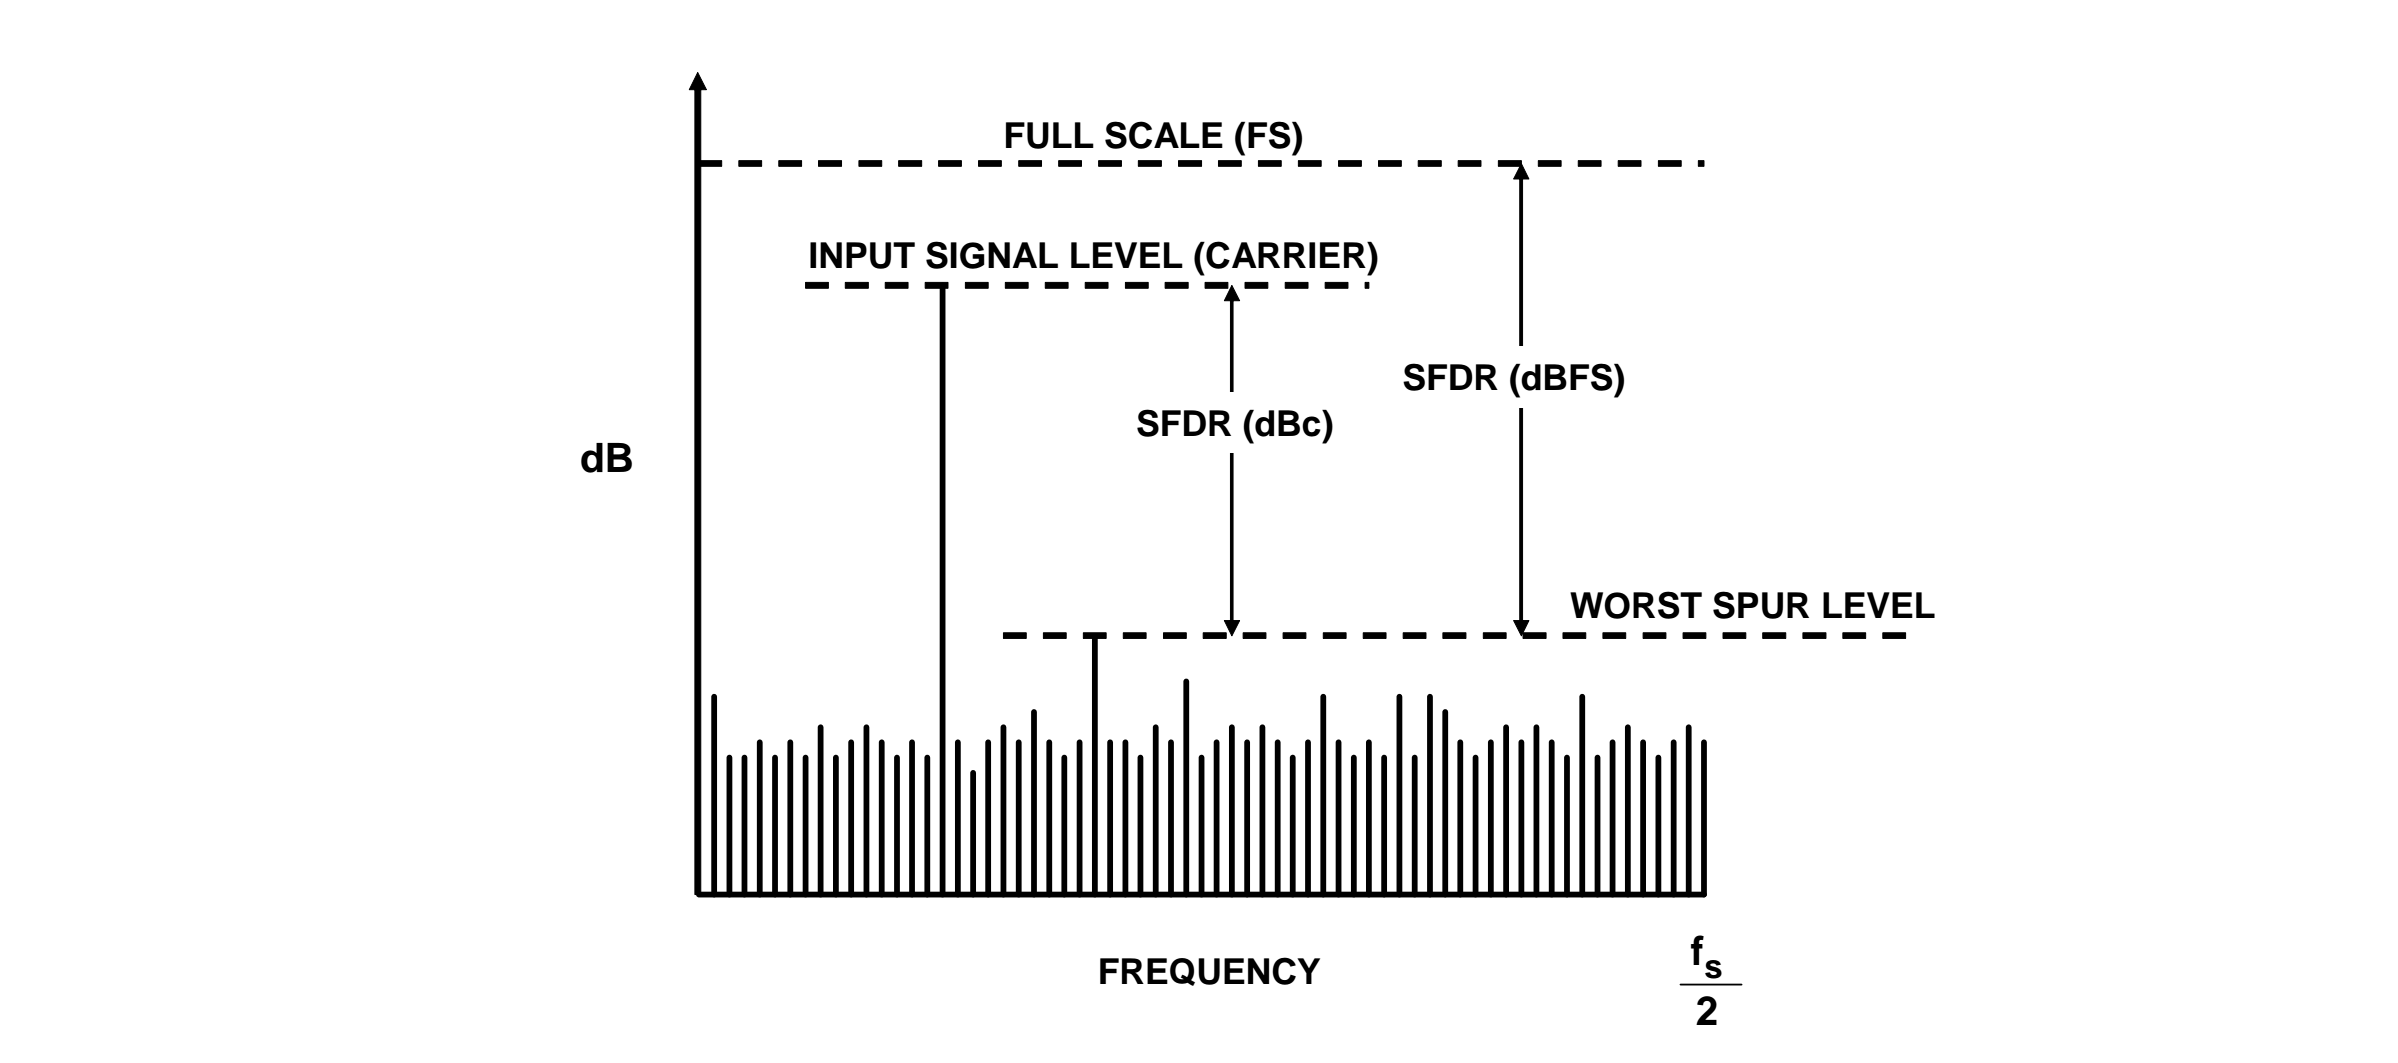
\includegraphics[width=\textwidth]{sfdr_plot}
  \caption{Spurious Free Dynamic Range [\citeauthor{understand_sinad}]}
  \label{fig:sfdr_plot}
\end{figure}

Finally the \emph{signal to noise and distortion ratio} (SINAD) is defined as the ratio of the RMS value of the input signal to the RMS value of all other spectral components including harmonics (but excluding DC):
\begin{align}
  \text{SINAD} = \frac{S_{rms}}{D_{rms}+N_{rms}}
\end{align}

SINAD is a good indicator of the dynamic performance of ADCs since it includes all components that make up noise and distortion. This parameter can also be related to the number of bits of the ADC using the theoretical ideal model of an ADC which assumes that only quantization noise exists and that it approximates AWGN \cite{improve_adc_res}:
\begin{align} \label{eq:SNR_ADC_dB}
  \text{SINAD(dB)} = (6.02 \cdot N_b) + 1.76
\end{align}
where $N_b$ is the number of bits of the ADC. It's important to note that \eqref{eq:SNR_ADC_dB} assumes a full-scale input signal as well. Finally, oversampling and averaging can be employed to reduce the in-band noise and hence increase the SINAD. In this case $N_b$ in \eqref{eq:SNR_ADC_dB} is replaced by the \emph{effective number of bits} (ENOB). Without going into the full detail, one can state a simple, but useful, rule of thumb:

\begin{displayquote}
  \emph{Each doubling of the sampling frequency will lower the in-band noise by 3 dB, and increase the resolution of the measurement by $1/2$ bit.}
\end{displayquote}

Note that whenever one is looking at a signal in the frequency domain, that's been obtained through an FFT, it's important to take into account the effects of the window used, namely the apparent attenuation caused by the signal not being contained within a single FFT bin (an effect known as \emph{scalloping loss}). Full analysis in beyond the scope of this thesis but can be consulted in \cite{harris_windows}.

SNR (or SINAD) can also be related to digital domain parameters. Closely related to the SNR is the $E_s$/$N_0$ parameter which is the ratio between the symbol energy and the noise spectral density. This parameter can be defined (in dB), and related to the SNR, as follows:
\begin{align}
  \frac{E_s}{N_0} (\text{dB}) & = 10\log_{10}\left(S\frac{T_{s}}{(N/B_n)}\right) \nonumber \\
                              & = 10\log_{10}\left(T_{s}F\left(\frac{S}{N}\right)\right) \nonumber \\
                              & = 10\log_{10}\left(\frac{T_{s}}{T}\right) + \text{SNR(dB)}
\end{align}
where
\begin{itemize}
  \item $T$ = Sampling period, in seconds
  \item $T_s$ = Symbol period, in seconds
  \item $S$ = Input signal power, in Watt
  \item $N$ = Noise power, in Watt
  \item $B_n$ = Noise bandwidth, in Hz $= F = 1/T$.
  \item $F$ = Sampling frequency, in Hz
\end{itemize}

$E_s/N_0$ can also be expressed in terms of the closely related ratio of the bit energy to the noise spectral density $E_b/N_0$ as
\begin{align}
  \label{eq:esn0}
  E_s/N_0 = E_b/N_0 + 10\log_{10}(k)
\end{align}
where $k$ is the number of \emph{information} bits per symbol. Note $k$ might be influenced by the size of the modulation alphabet or the code rate of an error-control code. For example, in a system using a rate-$1/2$ code and 8-PSK modulation, the number of information bits per symbol ($k$) is the product of the code rate and the number of coded bits per modulated symbol. Specifically, $(1/2) \log_2(8) = 3/2$. In such a system, three information bits correspond to six coded bits, which in turn correspond to two 8-PSK symbols.

Finally, and perhaps most important, is the notion of channel capacity famously introduced by Shannon \cite{shannon_capacity}. The information capacity of a channel of bandwidth $B$ (in Hz) with AWGN noise of power spectral density $N_0/2$ is given by
\begin{align}
  C = B\log_{2}\left(1+\frac{P}{N_0 B}\right)
\end{align}
where $P$ is the average transmitted power.

Note that the dependency on bandwidth $B$ is \emph{linear} but the dependency on SNR, $\frac{P}{N_0 B}$, is \emph{logarithmic}. This leads to an insightful conclusion:

\begin{displayquote}
  \emph{To increase the capacity of a communications systems it's easier to expand the bandwidth of the channel than to increase the transmitted power, for a given noise variance}.
\end{displayquote}

From this results it's possible to derive the familiar plots that relate SNR (or $E_b/N_0$) to bit-error rate (BER) which provide a very useful visual representation of the performance of digital modulations. \autoref{fig:PSK_BER_curves} shows a typical $E_b/N_0$ to BER curve for PSK modulations.

\begin{figure}[ht]
  \centering
  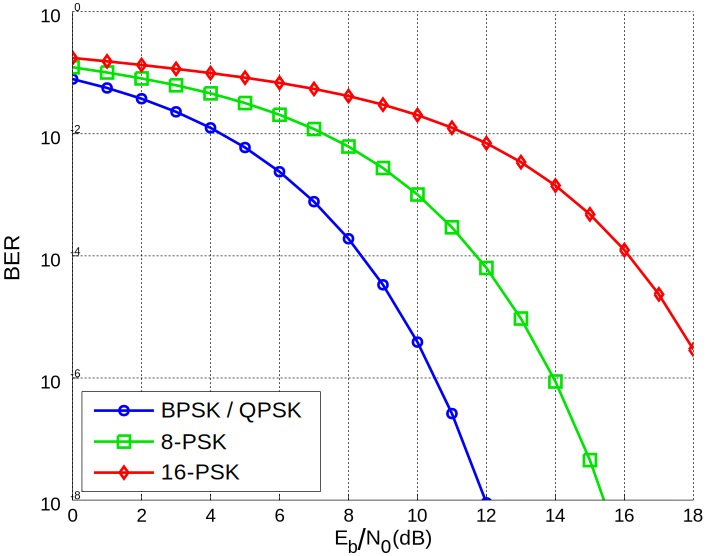
\includegraphics[width=0.75\textwidth]{PSK_BER_curves}
  \caption{Bit-error rate curves for BPSK, QPSK, 8-PSK and 16-PSK, AWGN channel [\citeauthor{image:ber_curve}]}
  \label{fig:PSK_BER_curves}
\end{figure}

Other parameters which are important in RF performance analysis, and are widely used for example in characterising PAs, are the 1-dB compression point (P1dB) and the third-order intercept point (IP3).

An amplifier usually provides a constant gain over a specific frequency range. If we represent the input power vs output power of an amplifier on a graph, we get a straight line (linear relationship) (i.e., output power = input power + gain), so, if the gain of an amplifier is 10 dB, then a 1 dBm input signal will result in an 11 dBm output signal and a 10 dBm input signal will result in a 20 dBm output signal. As the input power level increases, there comes a point where the output power of the amplifier no longer increases by the gain value (i.e., the amplifier output power starts to saturate). The P1dB is the output power level at which the gain decreases 1 dB from its constant value \cite{p1db}. Once an amplifier reaches its P1dB it goes into compression and becomes a non-linear device, producing distortion, harmonics and intermodulation products. Amplifiers should always be operated below the compression point. P1dB is one of the most important specifications for power amplifiers, as it is up to this point that we consider an amplifier to operate linearly. \autoref{fig:p1db} shows an illustration of the P1dB.

\begin{figure}[ht]
  \centering
  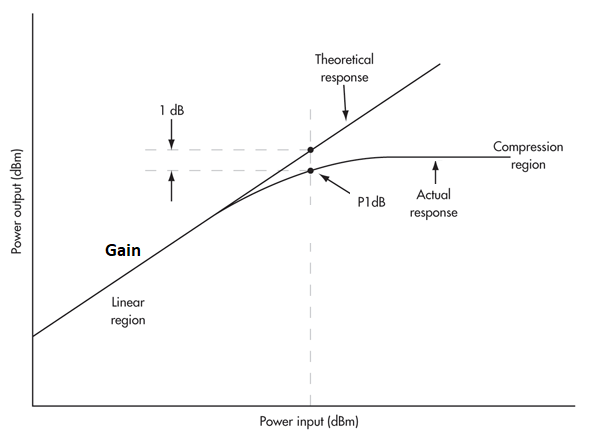
\includegraphics[width=0.6\textwidth]{p1db}
  \caption{1-dB compression point [\citeauthor{p1db}]}
  \label{fig:p1db}
\end{figure}

IP3 is a figure of merit based on the idea that the device nonlinearity can be modelled using a low-order polynomial, derived by means of Taylor series expansion \cite{iip3}. The third-order intercept point relates nonlinear products caused by the third-order nonlinear term to the linearly amplified signal, in contrast to the second-order intercept point that uses second-order terms. Two different definitions for intercept points are in use:
\begin{itemize}
  \item Based on harmonics: The device is tested using a single input tone. The nonlinear products caused by $n$-th-order nonlinearity appear at $n$ times the frequency of the input tone.
  \item Based on intermodulation products: The device is fed with two sine tones one at $f_1$ and one at $f_2$.  When you cube the sum of these sine waves you will get sine waves at various frequencies including $(2f_2-f_1)$ and $(2f_1-f_2)$.  If $f_1$ and $f_2$ are large but very close together then $(2f_2-f_1)$ and $(2f_1-f_2)$ will be very close to $f_1$ and $f_2$. This two-tone approach has the advantage that it is not restricted to broadband devices and is commonly used for radio receivers.
\end{itemize}
The intercept point is obtained graphically (\autoref{fig:iip3}) by plotting the output power versus the input power both on logarithmic scales (e.g., decibels). Two curves are drawn; one for the linearly amplified signal at an input tone frequency, one for a nonlinear product. On a logarithmic scale, the function $x^n$ translates into a straight line with slope of $n$. Therefore, the linearly amplified signal will exhibit a slope of $1$. A third-order nonlinear product will increase by 3 dB in power when the input power is raised by 1 dB. Both curves are extended with straight lines of slope $1$ and $n$ ($3$ for a third-order intercept point). The point where the curves intersect is the intercept point. It can be read off from the input or output power axis, leading to input (IIP3) or output (OIP3) intercept point respectively.

\begin{figure}[H]
  \centering
  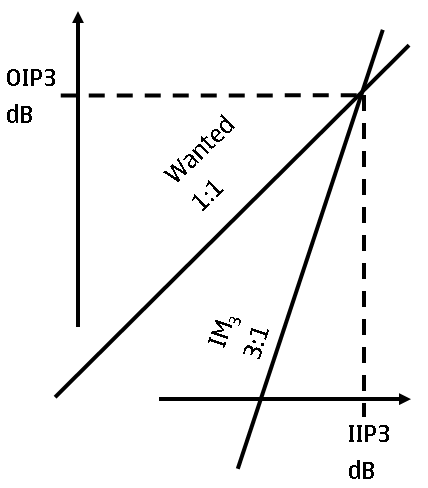
\includegraphics[width=0.4\textwidth]{iip3}
  \caption{Third-order intercept point [\citeauthor{iip3}]}
  \label{fig:iip3}
\end{figure}

Other important parameters, specific to quadrature systems, are \emph{IQ amplitude imbalance} and \emph{IQ phase imbalance}, which have to do with different gain and matching in the I and Q paths of a quadrature system. These will be discussed in more detail in \autoref{sect:sdr_system_architecture}.

%%%%%%%%%%%%%%%%%%%%%%%%%%%%%%%%%%%%%%%%%%%%%%%%%%%%%%%%%%%%%%%%%%%%%%%%%%%%%%%
\section{SDR System Architectures}
\label{sect:sdr_system_architecture}

This section covers some possible architectures in SDR systems, highlighting the main advantages and disadvantages of each one.

\subsection{Ideal SDR System}

The ideal SDR system (shown in \autoref{fig:ideal_sdr}) is one where the entire processing logic is encompassed within the DSP subsystem and the RF section simply needs to amplify and transmit/receive the signal. In this architecture the signal coming from/to the DAC/ADC is already at RF frequency so needs no further up/down conversion. Also, note the ADC and DAC include the anti-alias and reconstruction filters.

\begin{figure}[H]
  \centering
  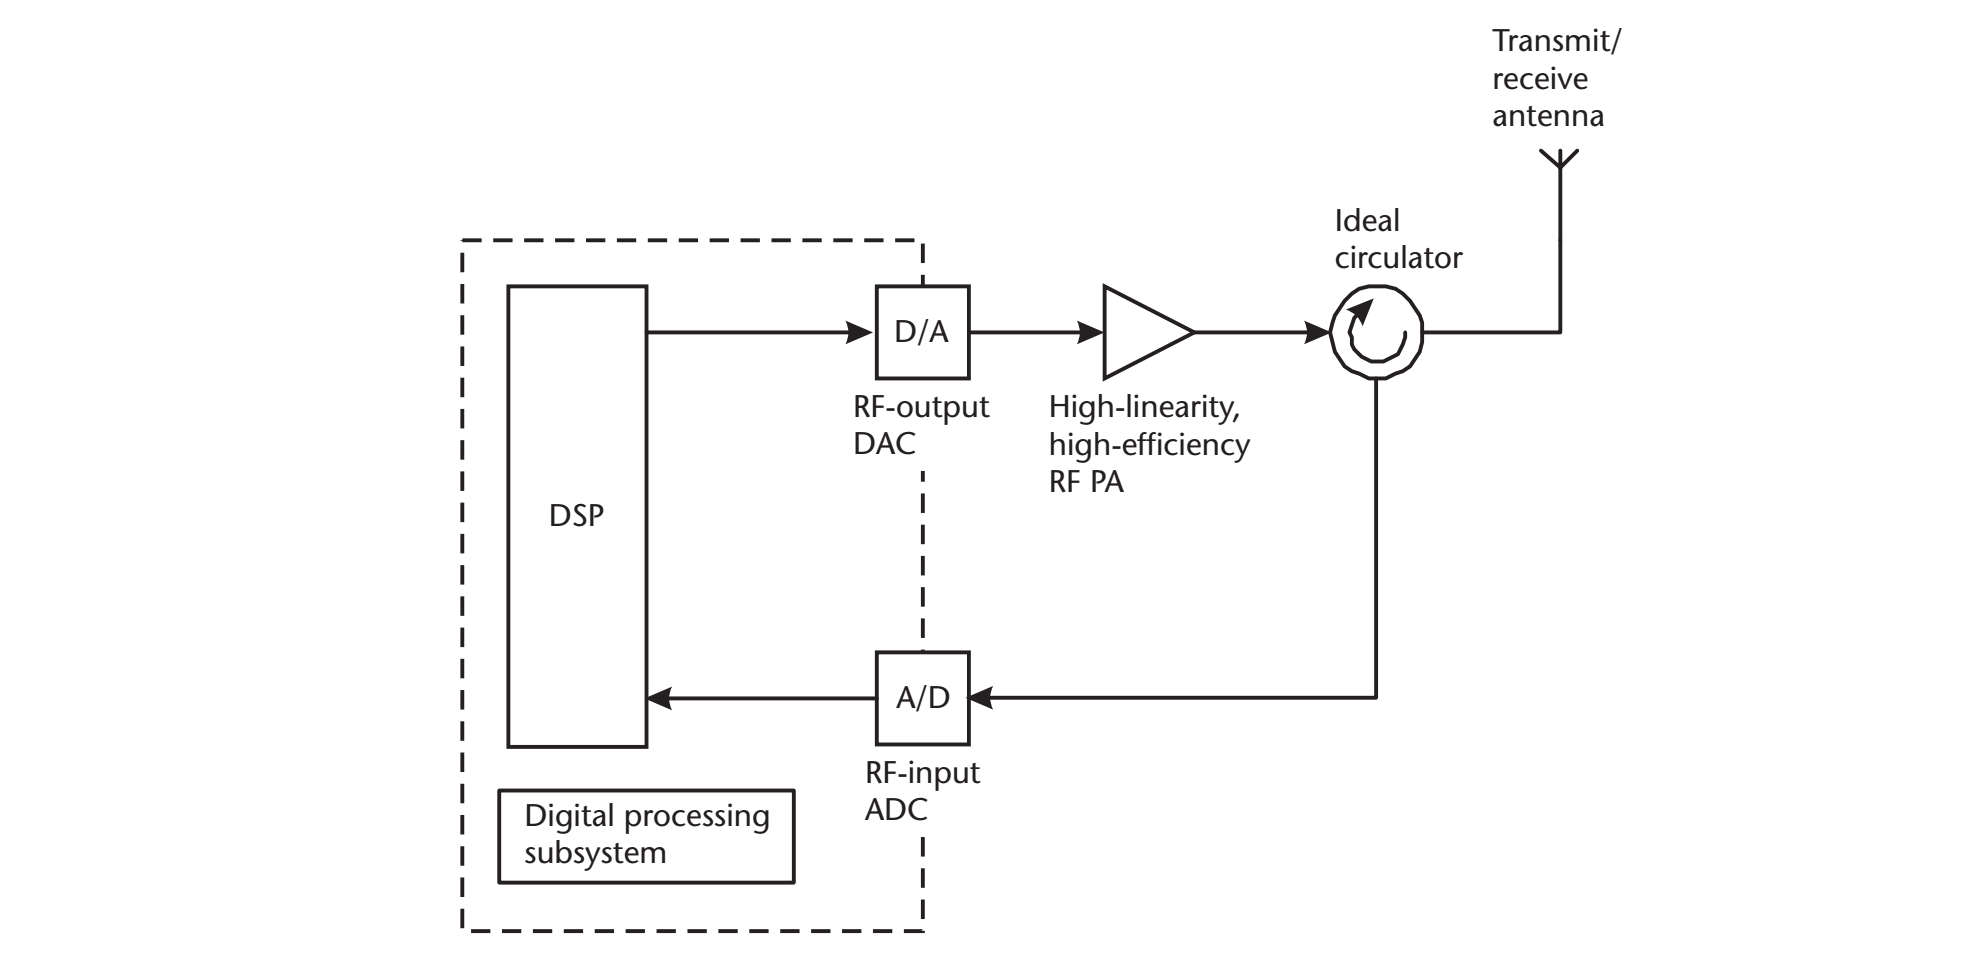
\includegraphics[width=\textwidth]{ideal_sdr}
  \caption[An ideal SDR system]{An ideal SDR system where the entire signal processing (including up/down conversion to the desired RF frequency) is achieved in the DSP subsystem [\citeauthor{rf_bb_techniques_sdr}]}
  \label{fig:ideal_sdr}
\end{figure}

Some of the clear advantages are:
\begin{itemize}
  \item Extremely simplified RF chain.
  \item Elimination of most of the analogue RF related problems such as DC offset, gain/phase imbalance in IQ systems, phase noise from oscillators, among others.
  \item Very high level of flexibility for implementing new protocols and/or when the processing power needs to be upgraded.
\end{itemize}

Unfortunately, technology has not evolved enough to make these systems cost effective. Their chief disadvantage is the fact that they rely on state-of-the-art high-speed ADC/DAC which are very expensive and power demanding (see \autoref{fig:adc12dj2700_power}), compared to a traditional up/down conversion RF chain (even considering the layout engineering effort involved in traditional RF chain design). Note that even if bandpass sampling is employed (which relaxes the sampling frequency requirements of the converters) the large analogue bandwidth necessary at the ADC input (often in the GHz range) is unavoidable if broadband is a requisite. Additionally, the realization of the anti-aliasing filter, which needs to provide sufficient attenuation in the stopband, while being tuned across the entire frequency range, is extremely challenging. As such, this architecture is necessarily reserved for systems where there are no budget restrictions. An RF sampling ADC characteristics page from a well-known vendor is shown in \autoref{fig:adc12dj2700_buy}. In this figure one can observe the very high sampling rate and input bandwidth, among other parameters. Note the full-scale input voltage of the ADC ($V_{FS}$) is just 0.8 V\textsubscript{pp}.

\begin{figure}[H]
  \centering
  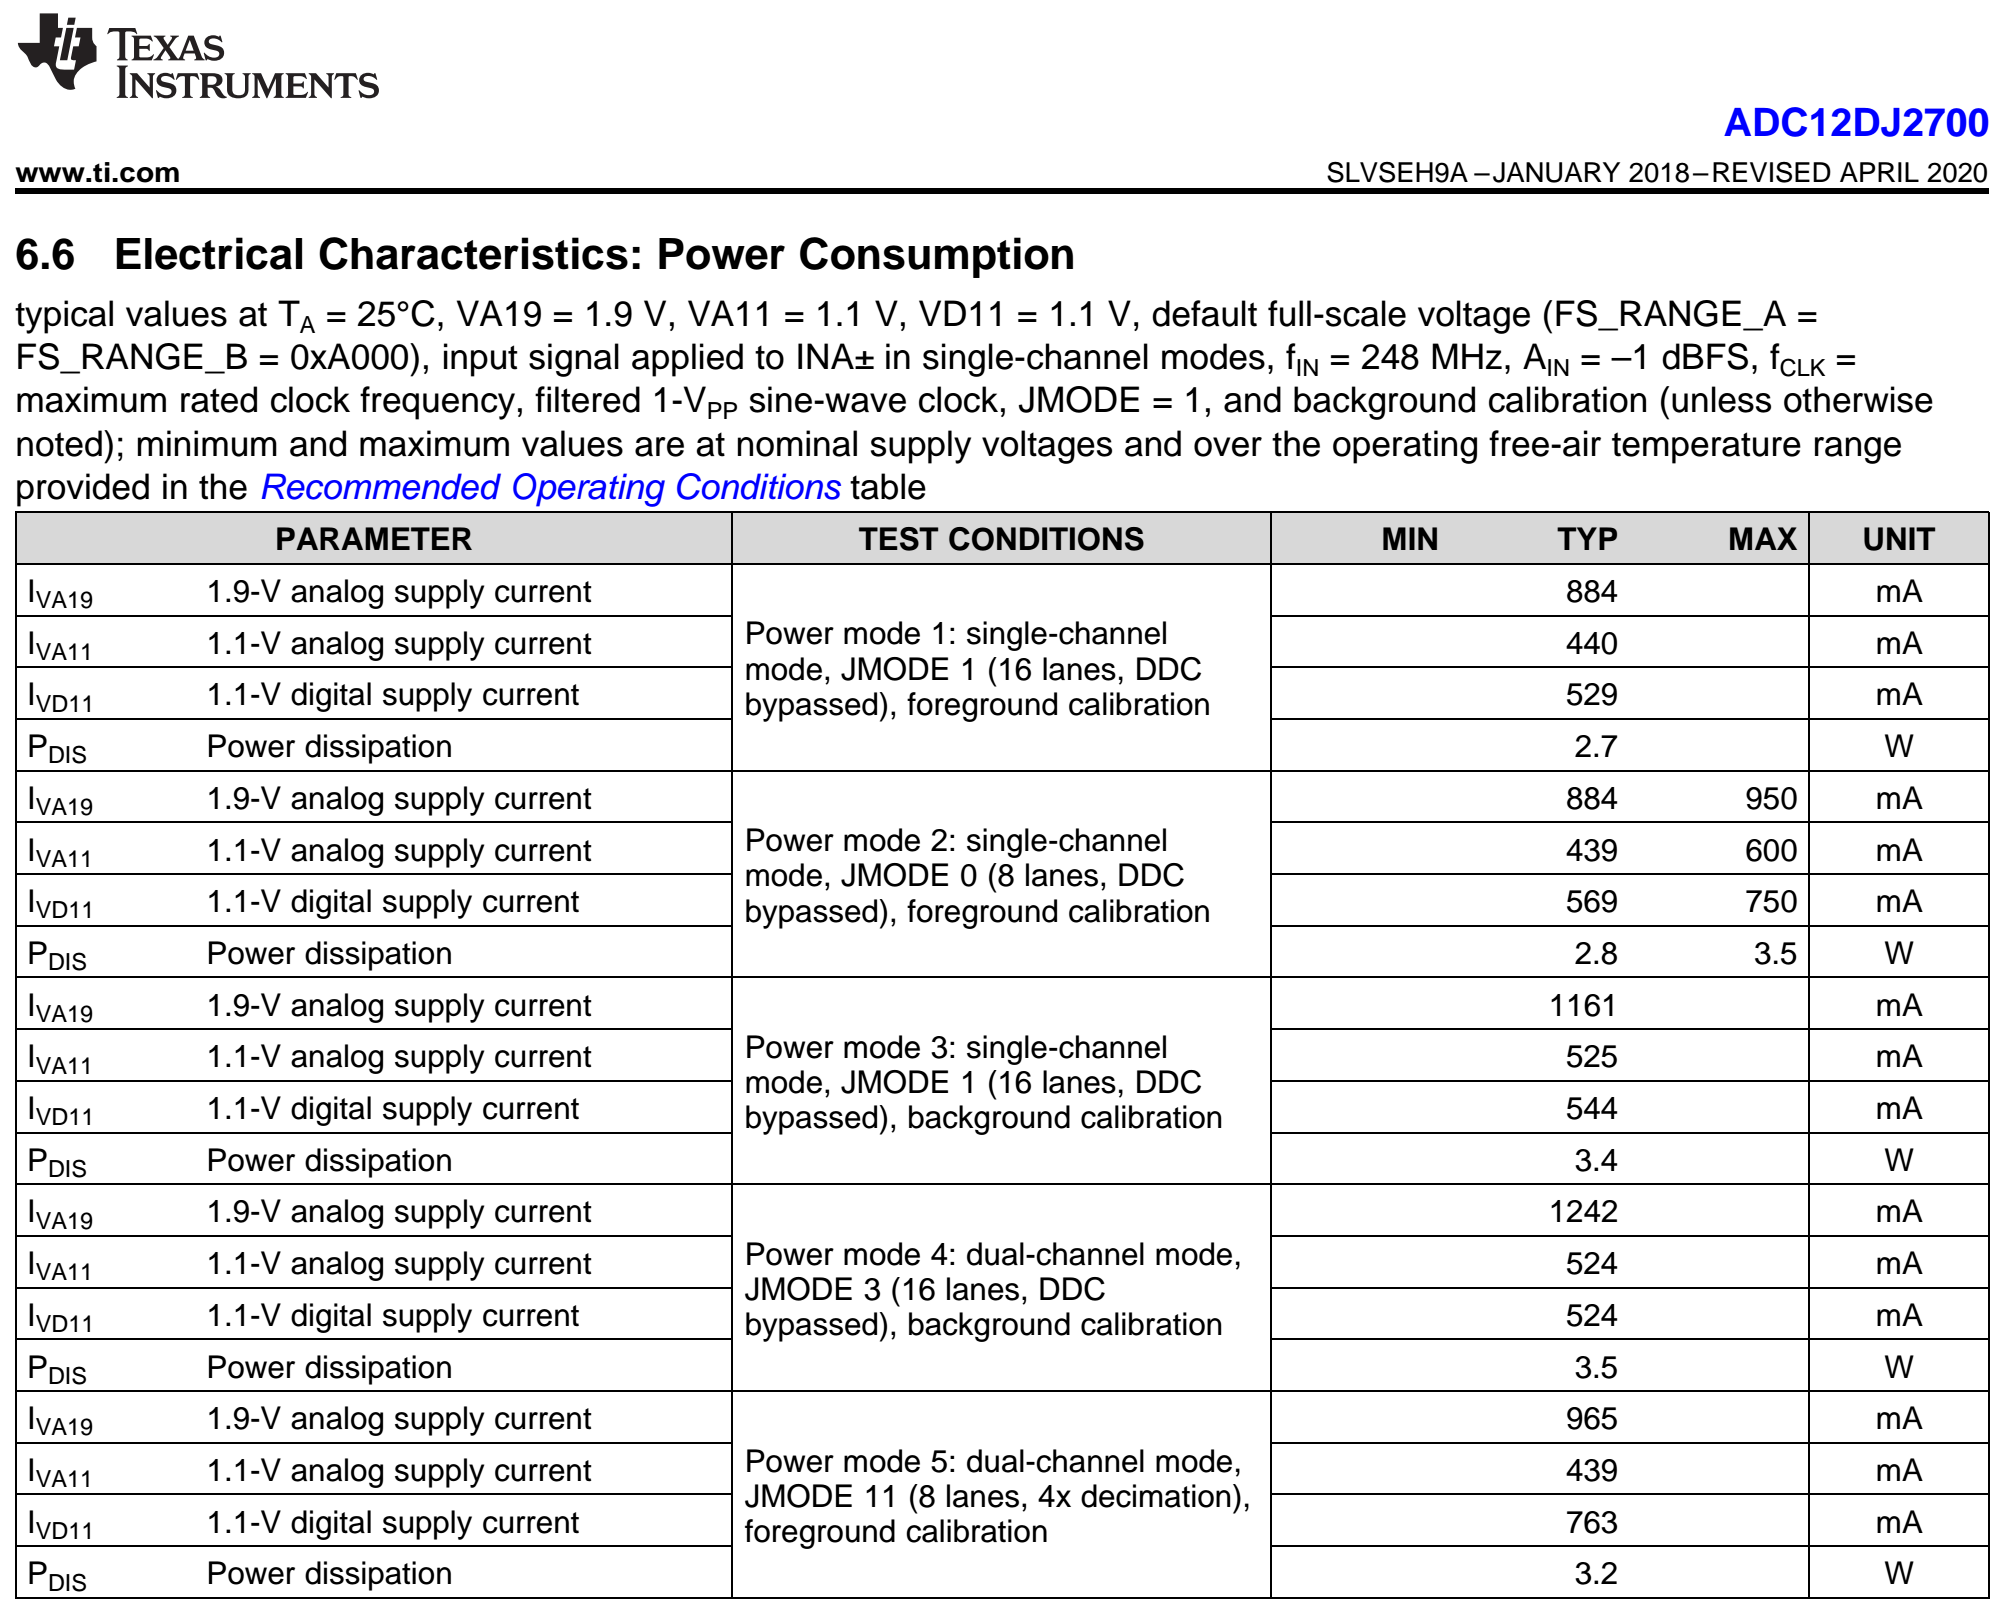
\includegraphics[width=\textwidth]{adc12dj2700_power}
  \caption[TI ADC12DJ2700 power consumption]{An extract from the TI ADC12DJ2700 datasheet, showing the power consumption of the device (from 2.7 W to 3.5 W depending on power mode)}
  \label{fig:adc12dj2700_power}
\end{figure}

\begin{figure}[H]
  \centering
  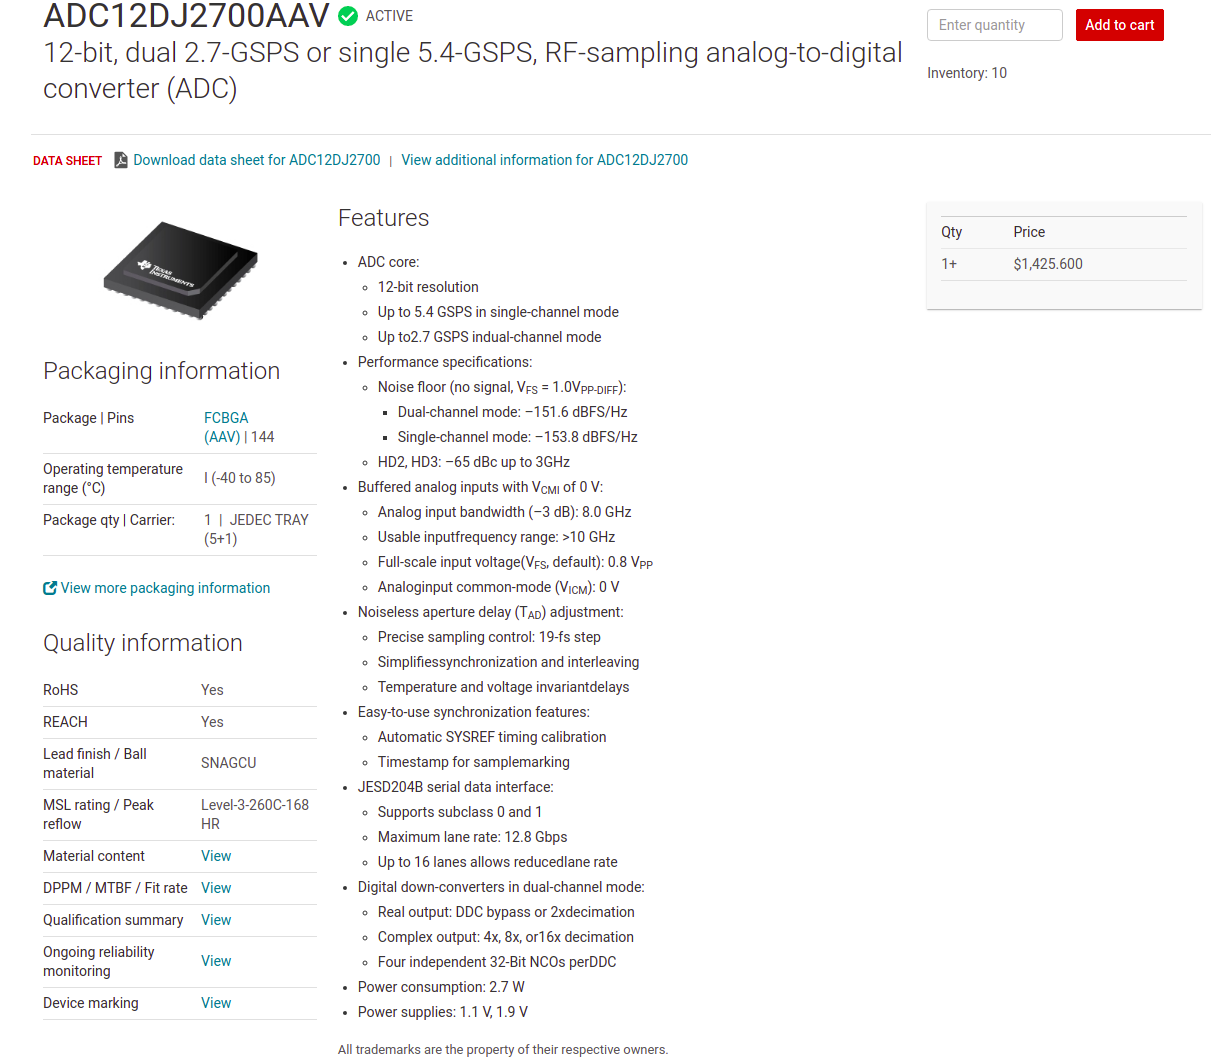
\includegraphics[width=\textwidth]{adc12dj2700_buy}
  \caption[TI ADC12DJ2700 specifications]{The TI ADC12DJ2700, a dual 2.7 GSPS, 12-bit RF sampling ADC which costs \$1425.60 per unit}
  \label{fig:adc12dj2700_buy}
\end{figure}

\subsection{Analogue Quadrature Receiver Architecture}
\label{sect:analogue_quadrature_receiver_architecture}

An alternative approach is seen in \autoref{fig:analog_quadrature_receiver} (only the receive path is shown for simplicity).

\begin{figure}[ht]
  \centering
  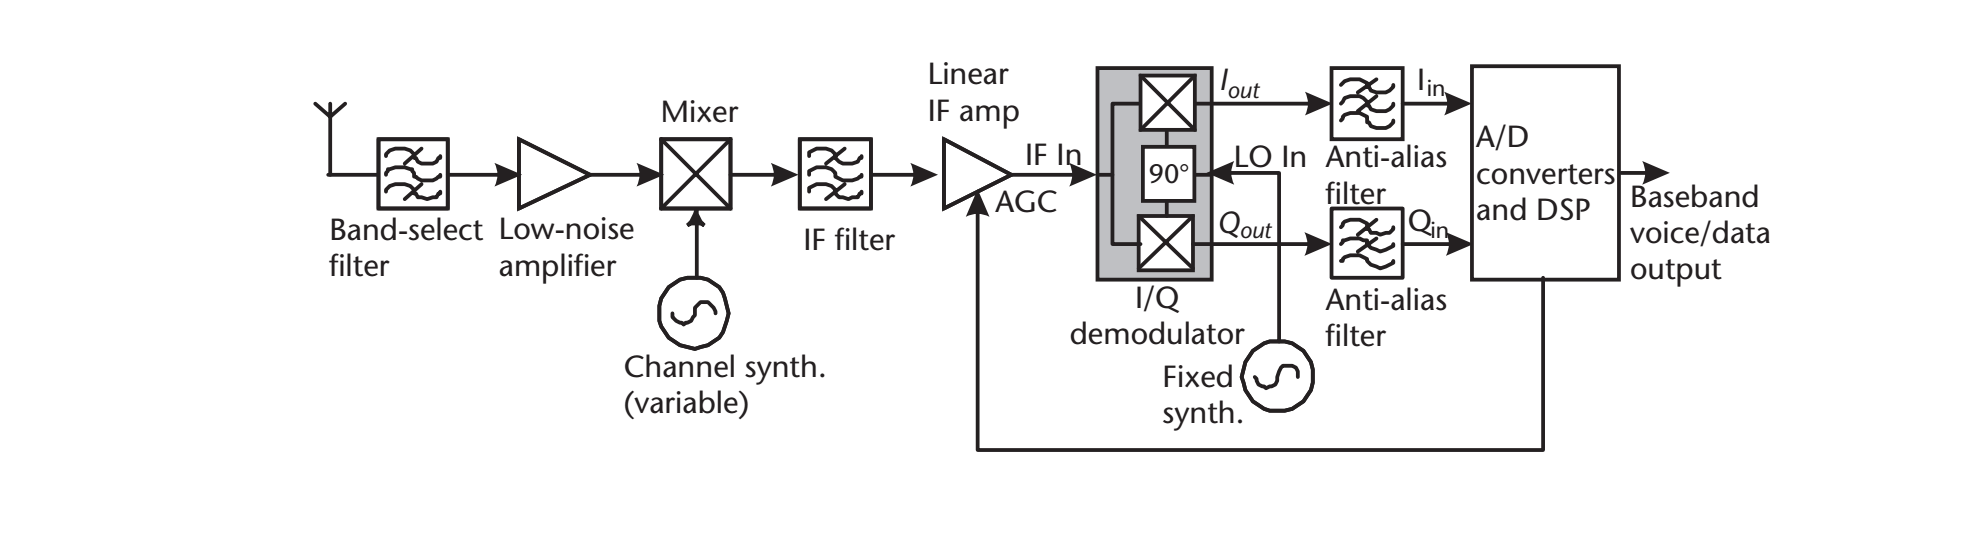
\includegraphics[width=\textwidth]{analog_quadrature_receiver}
  \caption[Analogue quadrature receiver design]{Analogue quadrature receiver design. A common implementation of SDR where the signal modulation and coding is performed in the DSP but the up/down conversion is achieved in the analogue domain [\citeauthor{rf_bb_techniques_sdr}].}
  \label{fig:analog_quadrature_receiver}
\end{figure}

In this case the RF chain needs to amplify and down-convert to IF. After that, the IF filter obtains the desired channel and then the signal is further down-converted to baseband, where the signal is low-pass filtered before being sampled by the ADC. The DSP finally performs the signal demodulation and decoding tasks such as constellation mapping and error correction decoding. The advantages in this architecture are:
\begin{itemize}
  \item Common and well understood architecture. For example, the IF section mitigates the DC offset problem caused by finite isolation between the input and the oscillator mixer ports (common problem in zero IF (ZIF) architecture, see \autoref{sect:zif_arch}).
  \item Transmit/receive path and ADC/DAC with more relaxed requirements can be implemented with relatively low-cost devices. ADC/DAC needs only to accommodate the baseband bandwidth and sampling frequency. Notice that it's becoming more common for the ADC/DAC blocks to include the anti-alias and reconstruction filters in one monolithic package, still maintaining low cost.
  \item Potential for implementing techniques such as oversampling to increase the ENOB and improve SNR.
\end{itemize}

The price to pay is:
\begin{itemize}
  \item Complex analogue path could lead to a slew of problems, especially if care is not taken in the layout phase. Potential for IQ gain and phase imbalance which need to be corrected.
  \item  Multi-stage amplification and filtering leads to the need to a complex mixed signal automatic gain controller (AGC) implementation where the DSP needs to control the analogue section gains in a feedback configuration to avoid saturation (note the figure shows the AGC controlling only the IF amplifier, but more often than not, it needs to control the whole chain, specially the LNA). Multiple oscillators can lead to strict clock requirements and complex architectures for coherent detection.
  \item Changes is system requirements such as different protocols and/or frequency ranges could potentially implicate a full hardware system re-design.
\end{itemize}

\subsection{Digital IF Receiver Architecture}

Perhaps a compromise between the two previous approaches is the \emph{Digital IF } architecture shown in \autoref{fig:digital_if_receiver}. In this realization, the analogue chain ends at the IF stage. The ADC samples directly at IF frequency and the conversion to baseband is performed in software by the DSP, together with the remaining demodulation, error correction and any other signal processing tasks. The IF frequency needs to be sufficiently high that some channel selection can be performed (for example 10 MHz being the minimum requirement, for 3GPP WCDMA, for example), but sufficiently low that a sensible A/D and DSP processing bandwidth results. This compromise is currently around the 10-50 MHz region, but continues to increase as A/D converter technology advances.

\begin{figure}[H]
  \centering
  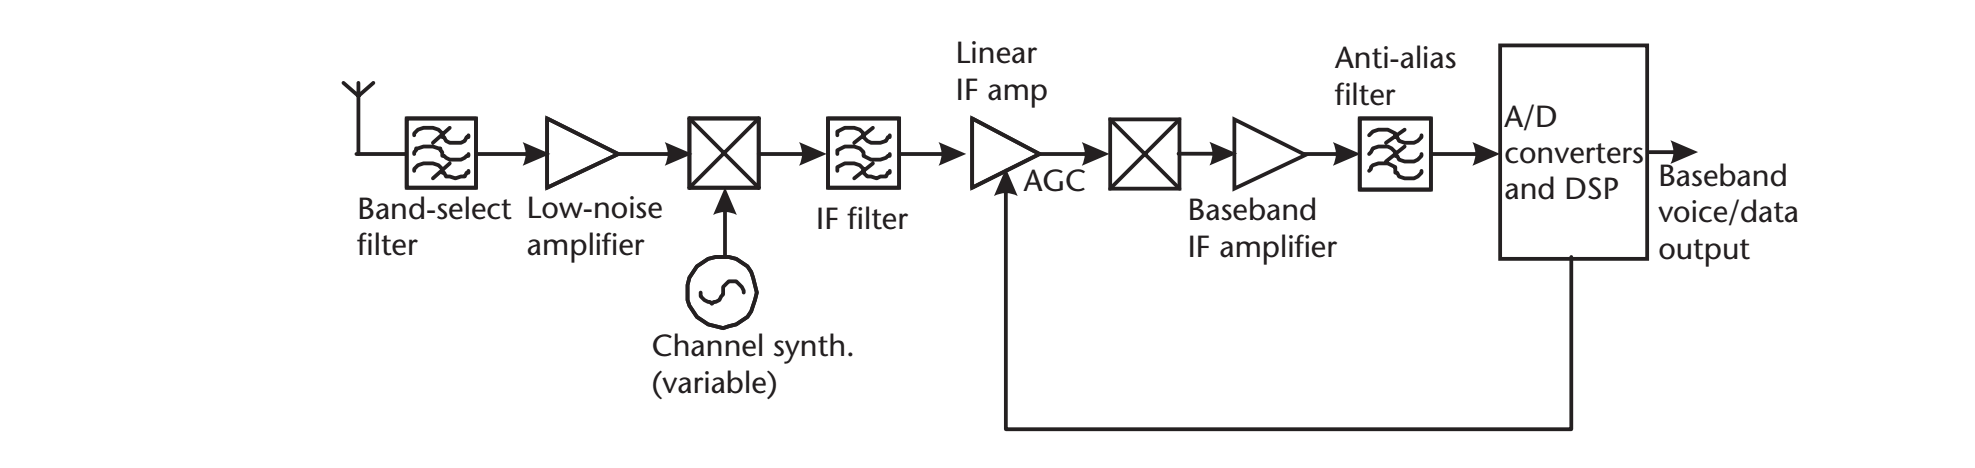
\includegraphics[width=\textwidth]{digital_if_receiver}
  \caption[Digital IF architecture]{Digital IF architecture. The analogue chain ends at the IF section. The ADC sample directly at the IF frequency and the downconvertion is then implemented in the DSP [\citeauthor{rf_bb_techniques_sdr}].}
  \label{fig:digital_if_receiver}
\end{figure}

There are some interesting advantages to this architecture:
\begin{itemize}
  \item Analogue section is confined to a single downconversion stage. The quadrature downconversion can be implemented in the DSP simply by mixing with quadrature (numerical) oscillator running at exactly $f_s/4$. This can be achieved by multiplying the digital IF samples by the periodic sequences [1, 0, -1, 0] for the in-phase channel and [0, -1, 0, -1] for the quadrature channel, therefore eliminating the problems mentioned in the analogue quadrature receiver architecture. This technique is shown in \autoref{fig:digital_quadrature_demod}.
  \item Simpler considerations for clocks and less analogue blocks to calibrate and control, lead to less requirements and complexity in the firmware.
  \item Potential for power consumption benefits  by having fewer analogue blocks and a simplified power saving logic.
\end{itemize}

The main disadvantages are:
\begin{itemize}
  \item Increased bandwidth necessary at the ADC to sample at IF, therefore possibly limiting other techniques such as oversampling.
  \item High-Q RF filtering section (typically a SAW filter) that needs to reject the image frequency at $f_c \pm f_i$.
\end{itemize}

\begin{figure}[ht]
  \centering
  
\includegraphics[width=\textwidth]{digital_quadrature_demod}
  \caption{Conceptual process of a digital quadrature demodulator [\citeauthor{rf_bb_techniques_sdr}]}
  \label{fig:digital_quadrature_demod}
\end{figure}

\subsection{Zero IF (ZIF) Receiver Architecture}
\label{sect:zif_arch}

In this architecture (also known as a \emph{homodyne receiver}), proposed by Colebrook in 1924 \cite{homodyne}, there is no IF stage, so the signal is directly converted to/from baseband. An example of this technique is shown in \autoref{fig:zif_receiver}.

\begin{figure}[H]
  \centering
  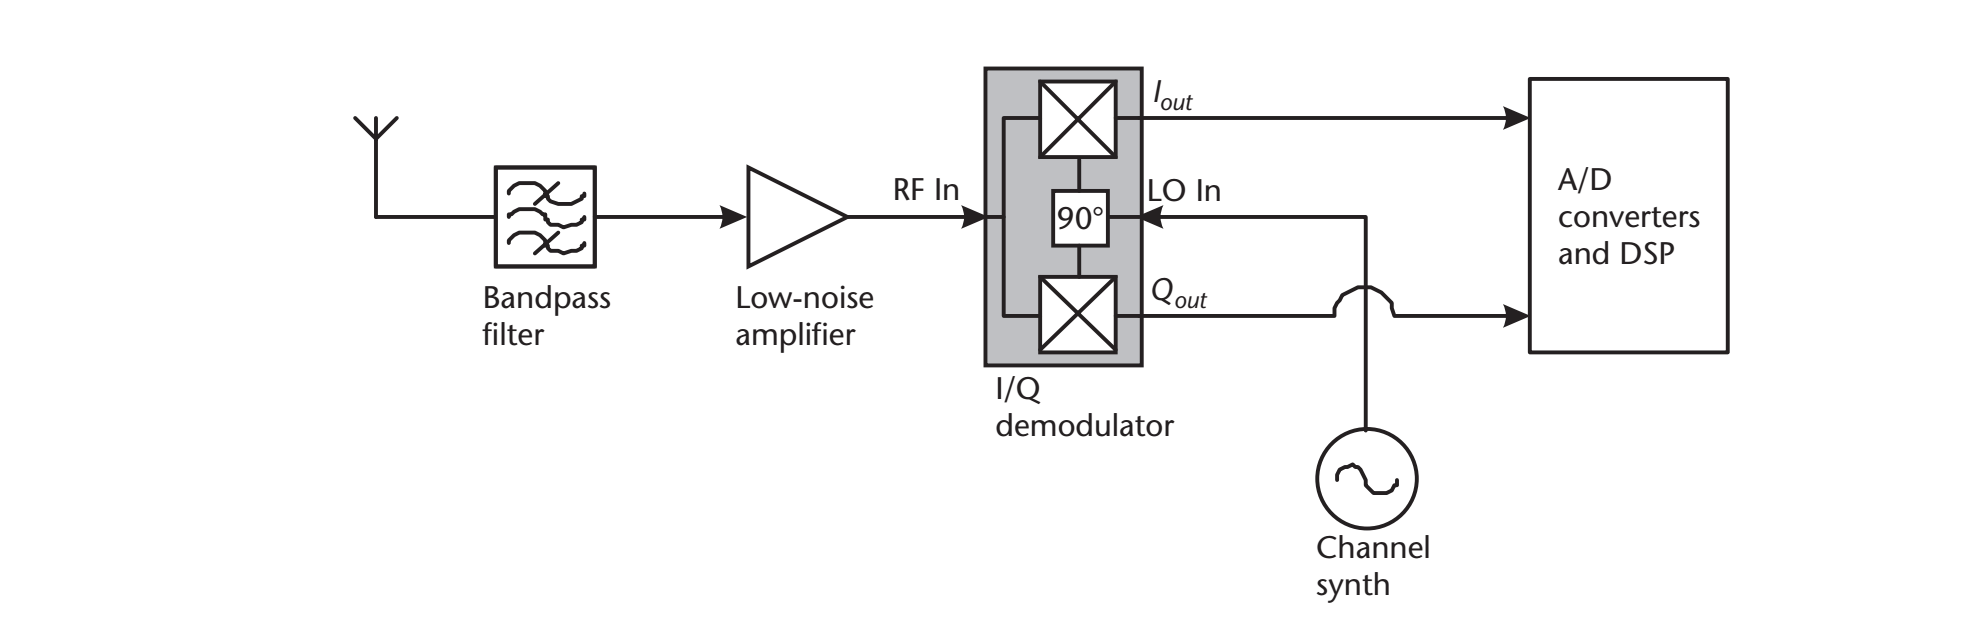
\includegraphics[width=\textwidth]{zif_receiver}
  \caption{Direct Conversion also known as Zero IF Architecture [\citeauthor{rf_bb_techniques_sdr}]}
  \label{fig:zif_receiver}
\end{figure}

This is potentially a very attractive option for the following reasons:
\begin{itemize}
  \item The use of digital filters allows for the implementation of far better channel selection filters than could be implemented in hardware at IF. In particular, tight specification linear-phase filtering is possible, which causes minimal disturbance to digital modulation schemes.
  \item The image frequency is in-band and hence the required image-rejection, based on the gain and phase balance of the IQ demodulator, is considerably reduced. Around 30-35 dB is acceptable for most systems.
  \item Only a single local oscillator signal is required, which is advantageous compared to heterodyne systems.
  \item No IF filter is required, hence saving cost and space and increasing the likelihood of achieving a single-chip solution.
\end{itemize}

It does, however, have a number of fundamental problems:
\begin{itemize}
  \item A high accuracy broadband quadrature network is required, to avoid IQ gain and phase imbalance.
  \item A DC offset appears at the centre of the baseband channel in I and Q and is usually quite high in level with respect to the weaker signals which the receiver may be required to demodulate. This is caused by finite isolation between LO and input ports in the mixer.
  \item LO re-radiation also causing DC offset. As the local oscillator appears on the wanted channel frequency and there is very little isolation between it and the antenna, significant levels of the LO signal can be re-broadcast.
  \item The use of a baseband IF results in problems with low-frequency noise appearing at the centre of the channel ($1/f$ noise).
  \item Second order (or second harmonic) distortion in the LNA or mixers can result in significant levels of second-order distortion appearing at (and around) DC.
\end{itemize}

%%%%%%%%%%%%%%%%%%%%%%%%%%%%%%%%%%%%%%%%%%%%%%%%%%%%%%%%%%%%%%%%%%%%%%%%%%%%%%%
\section{Signal Processing Realizations}
\label{sect:dsp_realizations}

SDR signal processing sections are implemented through employing various types of hardware platforms, such as GPPs, GPUs, DSPs, and FPGAs. Each of these platforms is associated with their own set of challenges. Some of these challenges are:
\begin{itemize}
  \item Utilizing the computational power of the selected hardware platform.
  \item Keeping the power consumption at a minimum.
  \item Ease of design process.
  \item Cost of tools and equipment.
\end{itemize}

\subsection{GPP}

One approach to realizing SDR platforms is using a GPP, such as x86/64 and ARM architectures. Examples of SDR platforms that utilize GPPs include Sora \cite{tan2011a}  and USRP \cite{usrp_product_selector}. A GPP is a digital circuit that is clock-driven and register-based and as such is capable of different processing functions \cite{microprocessors_and_microcontrollers}. This flexibility makes them extremely useful for unlimited number of applications, eliminating the need for building application specific circuits, and thus reducing the overall cost of running applications. GPPs also allow access to high-level programming languages and well-known frameworks and software packages, making them popular within the scientific community. From the performance point of view, GPPs are being enhanced rapidly, credited to technological advances in terms of CMOS technology \cite{lin2014a}, but also to the increase of the average number of instructions processed per clock cycle, achieved due the increase in multi-core GPP and exploring parallelism techniques within these cores \cite{ulversoy2010a}. Despite these advances, GPPs are still not convenient for high-throughput computing with real-time requirements, because of their sequential processing model \cite{kamal2003a}. The fact that the GPP often has to switch between different tasks when coupled with an operating system (OS), compromises its performance and can quickly reach saturation with frames becoming corrupted and being discarded. Moreover, wireless protocols require predictable performance in order to guarantee meeting timing constraints. However, conditional branch instructions in GPPs instruction sets lead to out-of-order execution, which makes it unfeasible to achieve predictability. To remedy the limitation of GPPs, researchers have proposed multiple solutions, one of which is the addition of co-processors, such as GPUs \cite{vachhani2015a}.

GPUs are processors specifically designed to handle graphics-related tasks and they efficiently process large blocks of streaming data in parallel and so can be used as co-processors for demanding operations, with the GPP typically acting as the control processor and relying on the GPU to do the intensive signal processing. SDR platforms comprised of both GPPs and GPUs are flexible and have a higher level of processing power. However, this results in a lower level of power efficiency (e.g., GPP's power efficiency is about 9 GFLOPS/W for single precision, compared to 20 GFLOPS/W for GPU \cite{v2014a}). The multi-core architectures and parallel processors in GPPs are the main attractive features, in addition to their relatively reasonable prices and reduced form factor. From an architectural perspective, GPUs have a number of advantages that makes them preferable solutions to applications such as video processing. In particular, they employ concepts such as\emph{single program multiple data} (SPMD) that allows multiple instruction streams to execute the same program, and \emph{single instruction multiple data} (SIMD) that allows an operation to be performed on multiple data points simultaneously.  Also their data load instructions are more efficient and they present a high computational density, where cache to arithmetic logic unit (ALU) ratio is low \cite{cope2010a}.

\begin{table}[ht]
  \caption{Performance of signal detection algorithm on GPP and GPU \cite{fi2017a}}
  \label{table:gpp_gpu_comparison}
  \centering
  \begin{adjustbox}{width=1\textwidth}
  \begin{tabular}{r|r|r|r}
    \toprule
    \multirow{2}{*}{\textbf{ADC Data Length (ms)}} & \multicolumn{3}{c}{Processing Platform of Signal Detection Algorithm} \\
    \multirow{2}{*}{} & \textbf{GPP Serial Processing (ms)} & \textbf{GPP Parallel Processing (ms)} & \textbf{GPU Parallel Processing (ms)} \\
    \midrule
    1    & 13.487    & 1.254    & 0.278 \\
    10   & 135.852   & 12.842   & 2.846 \\
    100  & 1384.237  & 131.026  & 29.358 \\
    1000 & 13946.218 & 1324.346 & 29.358 \\
    \bottomrule
  \end{tabular}
  \end{adjustbox}
\end{table}

In \autoref{table:gpp_gpu_comparison}, the authors of \cite{fi2017a} confirmed that the signal detection algorithm (which includes intensive FFT computations) shows a faster parallel processing in the case of GPU over GPP, while operating in real-time. This is due to the availability of \emph{cuFFT} library developed for NVIDIA GPUs for more efficient FFT processing \cite{cuda_toolkit}. With regards to the architectural advantage of GPUs, several thousand \emph{compute unified device architecture} (CUDA) cores can perform a single operation at the same time, as opposed to a few cores in the case of multi-core GPPs. Examples of using GPUs alongside GPPs to build SDR platforms is the work in \cite{szegvari2009a}, where the authors built a framework on a desktop PC, in addition to using a GPU, to implement an FM receiver. One thing to be aware is that, when both GPP and GPU are used for a SDR design, data transfer operations between GPP and GPU can be bottlenecks and cause performance loss \cite{li2014a}. Techniques introducing multi-stream scheduling for pipelining of the memory copy tasks have been recently suggested, to ensure no stalls in the pipeline, and thus enhancing processing parallelism \cite{accelerating_massive_mimo_uplink} \cite{millage2010a}. Finally, although the processing power of microprocessors is being constantly improved, balancing between sufficient computing power and a specific goal for energy consumption and cost, stays a very difficult task now and in the future.

\subsection{DSP}

A DSP is a particular type of microprocessor that is optimized to process digital signals \cite{rabiner1978a}. The DSP-based solution can be considered as a special case of GPP-based solutions, but due to its popularity and unique processing features, it deserves a separate discussion. An example of DSP-based SDR is the Atomix platform \cite{atomix} which utilizes TI TMS320C6670 \cite{unknown-h}. To help understand how DSPs are distinguished from GPPs, one should first note that both are capable of implementing and processing complex arithmetic tasks \cite{smith1997a}, like modulation/demodulation, filtering, and encoding/decoding, which are commonly used in applications that include speech recognition, image processing, and communication systems. DSPs, however, implement them more quickly and efficiently due to their architecture (e.g., RISC-like architecture, parallel processing) which is specifically optimized to handle arithmetic operations, especially multiplications. Since DSPs are capable of delivering high performance with lower power, they are better candidates for SDR deployment \cite{dyer1993a}, compared to GPPs. Examples of DSPs especially designed for SDR platforms are TI TMS320C6657 and TMS320C6655. These DSPs are both equipped with hardware accelerators for complex functions like the Viterbi and turbo decoders \cite{unknown-i}.

\subsection{FPGA-Based}

Another approach towards realizing SDRs is to use a programmable hardware such as FPGAs. An example of FPGA based SDR platform is the Xilinx Zynq-based implementation of IEEE 802.11ah described in \cite{80211ah_for_iot}, that uses this FPGA board to implement a complete communication system with channel coding. An FPGA is an array of programmable logic blocks, such as general logic, memory, and multiplier blocks, that are surrounded by a routing fabric, which is also programmable \cite{kuon2008a}. This circuit has the capability of implementing any design or function, with ease of updating it. Although FPGAs consume more power and occupy more area than ASICs, the programmability feature is the reason behind their increasing adoption in a wide range of applications. Another major difference is that, ASIC fabrication is expensive and requires a few months, whereas FPGAs can be quickly reprogrammed, and their cost is within a few tens to a few thousands of dollars, at most. The low-end product cycle, along with attractive hardware processing advantages, such as high speed performance, low power consumption, and portability, compared to processors such as GPPs and DSPs, present FPGAs as contenders that offer the best of both worlds \cite{kuon2008a}. This is due to the fixed architecture of the GPP, where not all functional units can be fully utilized, and the inherent parallelism of FPGAs and their dynamic architecture. In addition, despite having lower clock frequencies (up to about 500 MHz), FPGAs can achieve better performances due to their architectures which allow higher levels of parallelism through custom design \cite{sano2017a}. In a study by \cite{kestur2010a}, the authors compared the performance and power efficiency of FPGAs to that of GPPs and GPUs using double-precision floating point matrix vector multiplication. The results show that FPGAs are capable of outperforming the other platforms, while maintaining their flexibility.

Over the past decade, not only have FPGAs become significantly more powerful computationally, the availability of various toolsets have given them an additional advantage by making them more accessible. This is supported by the development of compilers that have the capability of generating register-transfer level (RTL) code, such as Verilog and VHDL, that is needed to run on FPGAs, from high-level programming languages. This process is typically referred to as \emph{high level synthesis} (HLS). Examples of such compilers include HDL Coder \cite{unknown-l} for MATLAB code \cite{matlab-a} and Xilinx HLS \cite{unknown-m}. HLS allows software engineers to design and implement applications, such as SDRs, on FPGAs using a familiar programming language to code, namely C, C++, SystemC, and MATLAB, without the need to possess a prior rich knowledge about the target hardware architecture. Further, FPGAs can achieve high performance while still consuming less energy than previously discussed processors \cite{choi2003a} (e.g., Intel Stratix 10 FPGA can achieve up to 100 GFLOPS/W \cite{altera2010a}, compared to 23 GFLOPS/W for NVIDIA GeForce GTX 980 Ti \cite{unknown-g}).

\subsection{Hybrid Design}

The fourth approach towards realizing SDRs is the hybrid approach, where both hardware and software-based techniques are combined into one platform. This is commonly referred to as the co-design or hybrid approach. Examples of SDRs that adopted the co-design approach include WARP \cite{khattab2008a} and CODIPHY \cite{dutta2013a}. Hardware/software co-design as a concept has been around for over a decade, and it has evolved at a faster rate in the past few years due to an increasing interest in solving integrated circuit design problems with a new and different approach. Even with GPPs becoming more powerful than ever, and with multi-core designs, it is clear that in order to achieve higher performance and realize applications that demand real-time processing, designers had to shift attention to new design schemes that utilize hardware solutions, namely, FPGAs and ASICs \cite{wolf2003a} \cite{micheli2001a}. Co-design indicates the use of hardware design methodology, represented by the FPGA fabric, and software methodology, represented by processors. As more applications, such as automotive, communication, and medical, grow in complexity and size, it has become a common practice to design systems that integrate both software (like firmware and operating system) and hardware \cite{teich2012a}. This has been made feasible in the recent years thanks to the advances in high-level synthesis and developing tools that not only have the capability to produce efficient RTL from software codes, but also define the interface between the both sides. The industry has realized the huge market for co-design, and provided various SoC boards that, in addition to the FPGA fabric, contain multiple processors. For example, the Xilinx Zynq board \cite{unknown-k} includes an FPGA fabric as well as two ARM Cortex-A9 processors \cite{unknown-p}. There are other reasons that make co-design even more interesting, including, faster time-to-market, lower power consumption (when optimized for this), flexibility, and higher processing speeds, as typically hardware in these systems is used as an acceleration to software bottlenecks \cite{windh2015a}. Adopting the co-design methodology in essence is a matter of partitioning the system into synthesizable hardware and executable software blocks.

A high-level comparison between three major design approaches as a guideline is presented in \autoref{table:sdr_approach_comparison}, focusing on the features that are important to SDR design. It shows that, while GPPs are easy to program and extremely flexible, they lack the processing power to meet specifications in real-time and are very inefficient in terms of energy consumption. To increase their performance, multiple cores with similar instruction sets are included in the same GPP platform to exploit parallelism and perform more operations per clock cycle. However, hardware replication (i.e., adding more cores to GPPs) may not necessarily translate to a higher performance. GPUs tackle this by offering the same control logic for several functional units. The sequential portion of the code runs on the GPP, which can be optimized on multi-core GPPs, while the computationally intensive portion runs on a several-hundred-core GPU, where the cores operate in parallel. Another example of a customized processor is DSP, which performs significantly better than GPPs, while at the same time maintaining the ease-of-use feature that GPPs possess, making them very attractive options. They are also more power efficient and better fit for signal processing applications. On the other hand, they are more expensive, which is the main trade-off. Finally, FPGAs combine the flexibility of processors and efficiency of hardware. FPGAs can achieve a high level of parallelism through dynamic reconfiguration, while yielding better power efficiency \cite{v2014a}. FPGAs are typically more suitable for fixed-point arithmetic, like signal processing tasks, but in the recent years their floating-point performance has increased significantly \cite{kestur2010a} \cite{underwood2004a}. However, the designers are expected to know a lot more about the hardware, which is sometimes a deterring feature.

\begin{table}[ht]
  \caption{Comparison of SDR design approaches [\citeauthor{DBLP:journals/corr/abs-1804-06564}]}
  \label{table:sdr_approach_comparison}
  \centering
  \begin{adjustbox}{width=1\textwidth}
  \begin{tabular}{>{\bfseries}l|c|c|c}
    \toprule
    & \textbf{GPP} & \textbf{DSP} & \textbf{FPGA} \\
    \midrule
    Computation        & Fixed Arithmetic Engines & Fixed Arithmetic Engines & User Configurable Logic\\
    Execution          & Sequential               & Partially Parallel       & Highly Parallel\\
    Throughput         & Low                      & Medium                   & High\\
    Data Rate          & Low                      & Medium                   & High\\
    Data Width         & Limited by Bus Width     & Limited by Bus Width     & High\\
    Programmability    & Easy                     & Easy                     & Moderate\\
    Complex Algorithms & Easy                     & Easy                     & Moderate\\
    I/O                & Dedicated Ports          & Dedicated Ports          & User Configurable Ports\\
    Cost               & Moderate                 & Low                      & Moderate\\
    Power Efficiency   & Low                      & Moderate                 & High\\
    Form Factor        & Large                    & Medium                   & Small\\
    \bottomrule
  \end{tabular}
  \end{adjustbox}
\end{table}

In a comparative analysis by \cite{betkaoui2010a}, authors studied the performance and energy efficiency of GPUs and FPGAs using a number of benchmarks in terms of targeted applications, complexity, and data type. The authors concluded that GPUs perform better for streaming applications, whereas FPGAs are more suitable for applications that employ intensive FFT computations, due to their ability to handle non-sequential memory accesses in a faster and more energy efficient manner. Similarly, in \cite{v2014a}, the authors review and report the sustainable performance and energy efficiency for different applications. One of their findings related to SDRs is that FPGAs should be used for signal processing without floating point, confirming aforementioned results. In addition, the authors in \cite{duan2011a} report that GPUs are ten times faster than FPGAs with regards to FFT processing, while authors in \cite{kestur2010a} demonstrate that the power efficiency of FPGAs is always better than GPUs for matrix operations.
